\documentclass[border=6pt]{standalone}
\usepackage{amsmath}
\usepackage{tikz}
\usetikzlibrary{decorations.pathreplacing,arrows.meta,calc,positioning}
\begin{document}
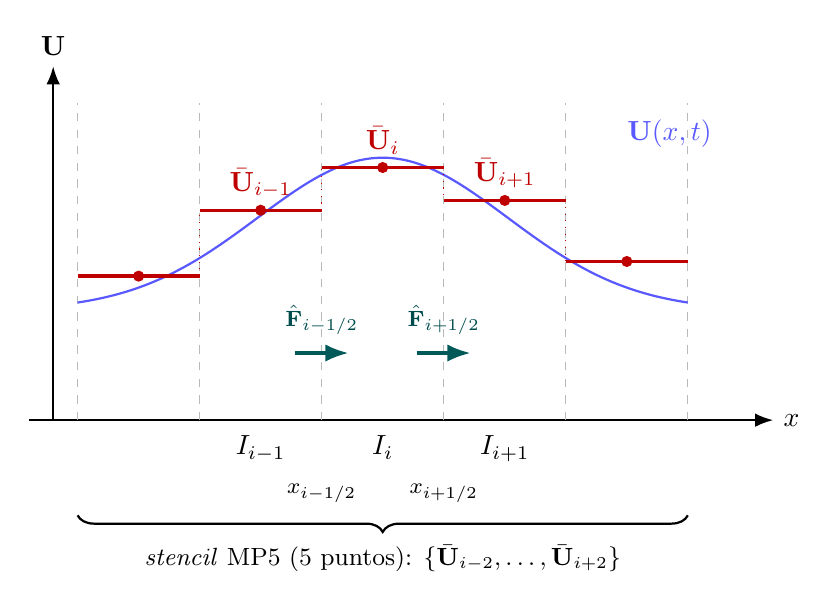
\begin{tikzpicture}[>=Latex,scale=1.55,
  cellavg/.style={very thick,red!75!black},
  flux/.style={->,very thick,teal!70!black}]

% --- ejes ---
\def\y0{0}
\draw[->,thick] (0.6,\y0) -- (6.7,\y0) node[right] {$x$};
\draw[->,thick] (0.8,\y0) -- (0.8,2.9) node[above] {$\mathbf{U}$};

% interfaces (x_{i±1/2}) en x=1..6
\foreach \x in {1,2,3,4,5,6}{
  \draw[gray!55,dashed] (\x,\y0) -- (\x,2.6);
}

% --- curva continua U(x,t) ---
\draw[thick,blue!65,smooth,samples=120,domain=1:6]
  plot (\x,{0.9+1.25*exp(-((\x-3.5)^2)/2.1)});
\node[blue!65] at (5.85,2.35) {$\mathbf{U}(x,t)$};

% --- promedios de celda (constantes a trozos) ---
% centros 1.5..5.5 ; alturas ~ promedio de la curva
\def\ha{1.18}\def\hb{1.72}\def\hc{2.07}\def\hd{1.80}\def\he{1.30}
\draw[cellavg] (1,\ha)--(2,\ha);
\draw[cellavg] (2,\hb)--(3,\hb);
\draw[cellavg] (3,\hc)--(4,\hc);
\draw[cellavg] (4,\hd)--(5,\hd);
\draw[cellavg] (5,\he)--(6,\he);
% escaloncitos verticales para que se vea piecewise-constant
\draw[red!75!black,thin,dotted] (2,\ha)--(2,\hb) (3,\hb)--(3,\hc) (4,\hc)--(4,\hd) (5,\hd)--(5,\he);

% etiquetas de promedios de celda
\node[red!75!black] at (2.5,\hb+0.22) {$\bar{\mathbf U}_{i-1}$};
\node[red!75!black] at (3.5,\hc+0.22) {$\bar{\mathbf U}_{i}$};
\node[red!75!black] at (4.5,\hd+0.22) {$\bar{\mathbf U}_{i+1}$};

% etiquetas de celdas I_i bajo el eje
\node[below] at (2.5,\y0-0.05) {$I_{i-1}$};
\node[below] at (3.5,\y0-0.05) {$I_{i}$};
\node[below] at (4.5,\y0-0.05) {$I_{i+1}$};

% etiquetas de interfaces
\node[below=1pt,font=\footnotesize] at (3,\y0-0.42) {$x_{i-1/2}$};
\node[below=1pt,font=\footnotesize] at (4,\y0-0.42) {$x_{i+1/2}$};

% --- flujos interfasiales (cruzan la interfaz) ---
\draw[flux] (2.78,0.55) -- (3.22,0.55);
\node[teal!60!black,font=\footnotesize] at (3,0.82) {$\hat{\mathbf F}_{i-1/2}$};
\draw[flux] (3.78,0.55) -- (4.22,0.55);
\node[teal!60!black,font=\footnotesize] at (4,0.82) {$\hat{\mathbf F}_{i+1/2}$};

% --- llave del stencil MP5 (5 celdas) ---
\draw[decorate,decoration={brace,amplitude=6pt,mirror},thick]
  (1,\y0-0.78) -- (6,\y0-0.78)
  node[midway,below=7pt,font=\small] {\emph{stencil} MP5 (5 puntos): $\{\bar{\mathbf U}_{i-2},\dots,\bar{\mathbf U}_{i+2}\}$};

% puntos del stencil
\foreach \cx/\hh in {1.5/\ha,2.5/\hb,3.5/\hc,4.5/\hd,5.5/\he}{
  \fill[red!75!black] (\cx,\hh) circle (1.3pt);
}
\end{tikzpicture}
\end{document}
